\setcounter{page}{0}
\vspace{-5em}
\chapter{Exposé}
\vspace{-2em}
\section{Problemstellung}
\vspace{-1em}
Im Teilprojekt B3 des Sonderforschungsbereichs Transregio 62 werden aktuell Regeln zur Bewertung der Ausgabegeräte verwendet.
Dies läuft im Moment wie folgt ab:
\begin{figure}[ht]
    \centering
    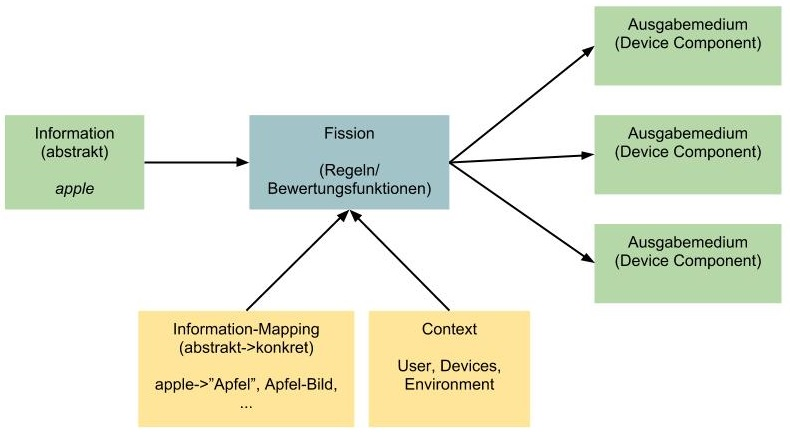
\includegraphics[width=.8\textwidth]{images/FissionUebersicht}
    \caption{\label{fission}Vereinfachte Übersicht der Funktionsweise der Fission}
\end{figure}

 Abstrakte Informationen werden vom Dialog-Manager an die Fission gesendet. Diese abstrakten Informationen werden dann von der Fission wie in Abbildung \ref{fission} zu sehen verarbeitet. Die Fission legt mittels eines Information-Mappings fest, wie die abstrakten Informationen als konkrete Informationen dargestellt werden können. So könnte zum Beispiel die abstrakte Information \emph{apple} sowohl als Text als auch als Bild dargestellt werden. Diese konkreten Daten werden dann im Bezug auf die vorhandenen Kontextinformationen (wie  User-, Environment- oder Device-Context bewertet.
Die Bewertung basiert auf unterschiedlichen Bewertungsfunktionen. Eine Funktion repräsentiert dabei eine gestalterisch bewertete Aussage, z.\,B.: \glqq Es ist sehr gut den akustischen Kanal einzusetzen wenn der Nutzer blind ist.\grqq \ Außerdem besitzt jede Regel einen Funktionswert, der positiv oder negativ sein kann. Alle Regeln werden dann auf alle Kombinationen aus konkreten Informationen und Ausgabemedien(Devices) angewendet. Dabei kann jede Regel mit einer unterschiedlichen Gewichtung in die Bewertung einfließen. Die Gewichtung geht aus dem Kontext hervor.
\linebreak
Dieser Ansatz der Bewertung hat vermutlich exponentielle Laufzeitkomplexität. Davon ausgehend, dass bereits ein weitestgehend optimaler Algorithmus genutzt wird um die Bewertung der Regeln zu berechnen soll dieser Ansatz nun evaluiert werden. Dies dient dazu Aussagen über den Einfluss der Variablen auf die Laufzeit treffen zu können. 


\section{Geplantes Vorgehen}
\vspace{-1em}
Das Vorgehen kann in drei Teile, die Analyse, Evaluation und Bewertung des aktuellen Ansatz aufgeteilt werden. Ziel ist es klare Aussagen über das Laufzeitverhalten der Fission bei sich ändernden Variablen (siehe hierzu auch Evaluation) zu treffen.
\vspace{-2em}
\subsection{Analyse}
\vspace{-1em}
Hierbei geht es um eine theoretische Betrachtung des aktuell gewählten Ansatzes. Zunächst wird das Problem und die dafür geeigneten Algorithmen klassifiziert und ihre  theoretische Laufzeitkomplexität bestimmt. Auf Basis dieser Analyse werden dann bei der Evaluation zu prüfende Werte festgelegt, die ein möglichst idealer Algorithmus einhalten soll. Es sollten außerdem für die Evaluation nötigen Kriterien definiert werden, die dann wiederum wichtigen Einfluss auf die Planung haben.
\vspace{-2em}
\subsection{Evaluation}
\vspace{-1em}
Zur Evaluation soll ein Tool entwickelt werden, welches den Bewertungsalgorithmus der Fission durch einen Lasttest unabhängig untersucht, dabei soll es möglich sein unterschiedliche Variablen (Problemgrößen) verändern zu können: Abstrakte Daten, Daten-Mappings, Kontext (User, Environment, Device). Außerdem soll das Evaluations-Tool in der Lage sein die Laufzeiten zu erfassen und angemessen zu protokollieren. Die genauen Anforderungen an das Evaluations-Tool gehen aus der Analyse hervor. Diese Ergebnisse sind Grundlage für die Planung der Test-Settings. Diese sollen durchlaufen und deren Laufzeiten protokolliert und in einem Folgeschritt analysiert werden.

\vspace{-2em}
\subsection{Auswertung}
\vspace{-1em}
Im Anhschluss an die Simulation sollen die daraus resultierenden Ergebnisse evaluiert werden. Ziel ist es Richt- bzw. Grenzwerte für die maximale Anzahl an Variablen die den Bewertungsalgorithmus der Fission beeinflussen zu empfehlen.
Eventuell kann aus den Ergebnissen und der Analyse auch eine Anpassung des Algorithmus empfohlen werden.


\section{Geplante Gliederung}
\vspace{-1em}
\begin{itemize}
    \item  Motivation
    \item  Beschreibung der Problemstellung
    \begin{itemize}
        \item  Regeln/Evaluationsfunktionen
        \item  Kontext
        \item  Abstrakte Informationen und Informationsmapping
    \end{itemize}
    \item  Evaluationsansätze vergleichbarer Systeme
    \item  Theoretische Analyse
    \begin{itemize}
        \item  Beschreibung des aktuellen Ansatz (Algorithmus)
        \item  Theoretische Bewertung
        \item  Evtl. Vergleich mit ähnlichen Lösungen
    \end{itemize}
    \item  Evaluation
    \begin{itemize}
        \item  Planung
        \item  Entwicklung Evaluationstool
        \item  Durchführung
    \end{itemize}
    \item  Auswertung und Diskussion
     \begin{itemize}
     	\item  Zusammenfassung
     	\item  Diskussion
        \item  Evtl. Verbesserungsansätze identifizieren
    \end{itemize}
\end{itemize}


\section{Zeitabschätzung}
Bei einer Bachelorarbeit im Umfang von 12 LP können 40 Tage für die eigentliche Durchführung geplant werden. Aus der Gliederung ergibt sich also folgende Zeitabschätzung:
\begin{table}[h]
    \centering
    \begin{tabular}{|l|l|l|}
    	\hline
        Arbeitspaket & Zeit in Tagen \\
        \hline
        Beschreibung der Problemstellung & 2 Tage \\
        Analyse & 5 Tage \\
        Evaluation - Planung & 7 Tage \\
        Evaluation - Entwicklung Evaluationstool & 12 Tage \\
        Evaluation - Durchführung & 5 Tage \\
        Auswertung - Zusammenfassung & 7 Tage \\
        Auswertung - Diskussion & 2 Tage \\
        Auswertung - Evtl. Verbesserungsansätze identifizieren & 3 Tage \\
        \hline
        Gesamt & 40 Tage \\
        \hline
        
    \end{tabular}
\end{table}
